% ============PREAMBLE SECTION==========================================
%+++++++++++++++++++++++++++++++++++++++++++++++++++++++++++++++++++++++
\documentclass[12pt]{article}
\usepackage{geometry}                % See geometry.pdf to learn the layout options. There are lots.
\geometry{letterpaper}                   % ... or a4paper or a5paper or ... 
%\geometry{landscape}                % Activate for for rotated page geometry
\usepackage[parfill]{parskip}    % Activate to begin paragraphs with an empty line rather than an indent
\usepackage{daves,fancyhdr,natbib,graphicx,dcolumn,amsmath,lastpage,url}
\usepackage{amsmath,amssymb,epstopdf,longtable}
\DeclareGraphicsRule{.tif}{png}{.png}{`convert #1 `dirname #1`/`basename #1 .tif`.png}
\pagestyle{fancy}
\lhead{Student Name: \_\_\_\_\_\_\_\_\_\_\_\_\_\_\_\_\_\_\_\_\_\_\_\_\_\_\_\_\_\_\_\_\_\_\_\_\_\_\_\_\_\_\_\_\_ }
\rhead{FALL 2024}
\lfoot{CE 3354 Engineering Hydrology }
\cfoot{EXAM 1}
\rfoot{Page \thepage\ of \pageref{LastPage}}
\renewcommand\headrulewidth{0pt}

% other
\usepackage{paralist}  % need to modify standard enumerate blocks
%=========Longtable environment
\usepackage{setspace}                % allow single and double space environment
\usepackage{longtable}                % allow table to span multiple pages
\usepackage{caption}                    % consistent caption package
\usepackage{url}					% Ubiquitious url formatting package
%===========

\DeclareGraphicsRule{.tif}{png}{.png}{`convert #1 `dirname #1`/`basename #1 .tif`.png}
\pagestyle{fancy}
\lhead{Student Name: \_\_\_\_\_\_\_\_\_\_\_\_\_\_\_\_\_\_\_\_\_\_\_\_\_\_\_\_\_\_\_\_\_\_\_\_\_\_\_\_\_\_\_\_\_ }
\rhead{FALL 2024}
\lfoot{CE 3354 Engineering Hydrology }
\cfoot{EXAM 1}
\rfoot{Page \thepage\ of \pageref{LastPage}}
\renewcommand\headrulewidth{0pt}
%++++++++++++++++++++++++++++++++++++++++++++++++++++++++++++++++++++++++++
%============================================================================
\begin{document}

\begingroup
\begin{centering}
\textbf{CE 3354 Engineering Hydrology} \\
\textbf{Exam 1 (Alternate) , Fall 2024}\\
\end{centering}
~\\
Students should write their name on \textbf{all sheets of paper}.  \newline 
Students are permitted to use the internet to help answer questions.  \newline 
Students are permitted to use their own notes and the textbook.\newline 
Students are \textbf{forbidden} to \textbf{communicate with other people} during the examination.
\endgroup

\begin{enumerate}
\item Provide short answers to the following questions:
\begin{enumerate}[a)]
\item What is a ``watershed?''
~\newline
~\newline
~\newline
~\newline
\item What is ``excess precipitation ?''
~\newline 
~\newline
~\newline
~\newline
~\newline
\item  What is ``a hyetograph?''
~\newline
~\newline
~\newline
~\newline
~\newline
\item What is  ``a hydrograph?''
~\newline
~\newline
~\newline
~\newline
~\newline
\item What is ``an intensity-duration-frequency curve?''
~\newline
~\newline
~\newline
~\newline
~\newline
\end{enumerate}
\clearpage
\item  Figure \ref{fig:topoMap.jpg} is a hand-drawn topographic map of somewhere in Texas.  The drawn contour interval is 20 feet.  Most of the contours are labeled --- the South-East corner is at elevation $\approx{} 550 ft$.  The North-West corner is at elevation $\approx{} 650 ft$.   
\\

\begin{figure}[h!] %  figure placement: here, top, bottom, or page
   \centering
   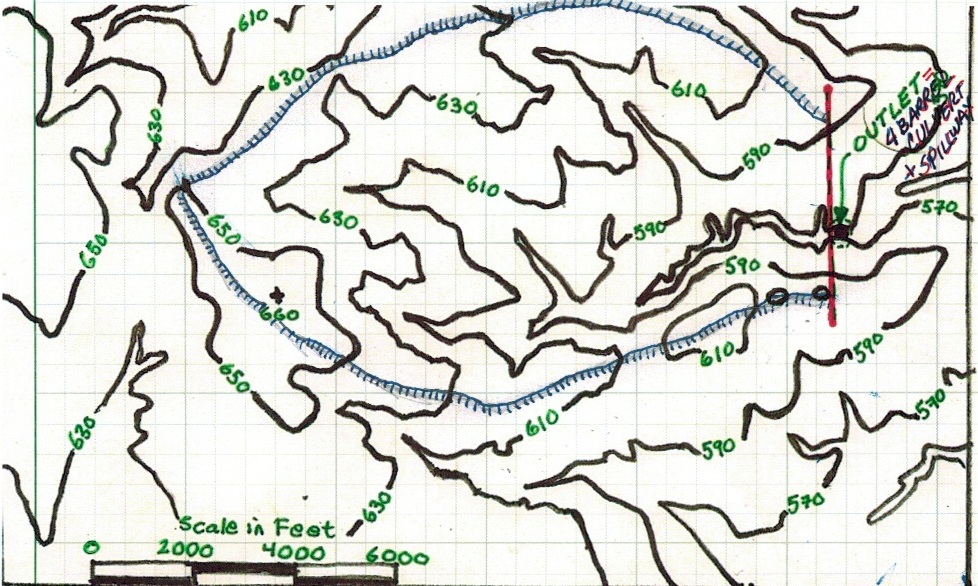
\includegraphics[width=6.5in]{topoMap.jpg} 
   \caption{Topographic Map of a portion of the Earth.  Elevations and linear distances are in $feet$. North (by convention) is up.}
   \label{fig:topoMap.jpg}
\end{figure}

Useful unit conversions:
\begin{itemize}
\item $43560~ ft^2 = 1 ~acre$
\item $640 ~acres = 1 ~square~mile$
\item $5280 ~feet = 1 ~mile$
\end{itemize}
\clearpage
\begin{enumerate}[a)]
\item What is the area in $ft^2$, $acres$, and $mi^2$ depicted by the map \footnote{The area of the whole rectangle} on Figure \ref{fig:topoMap.jpg} ?  Explain by sketch or words how you computed the area. 
~\newline
~\newline
~\newline
~\newline
~\newline
~\newline
~\newline
~\newline
\item Locate the highest point depicted on the map.  Circle this point. 
\item What is the numerical value of elevation in feet of this location (read from map)?
~\newline
~\newline
~\newline
~\newline
\item What is the numerical value of the contour line that encloses this location (read from map --- the point is higher than this contour, but the point is entirely enclosed by a contour).
~\newline
~\newline
~\newline
~\newline
\item Lightly shade the area within the contour.  
\item Determine the area in in $ft^2$, $acres$, and $mi^2$ of the shaded region.  Again explain by sketch or words how you computed the area.
~\newline
~\newline
~\newline
~\newline
~\newline
~\newline
~\newline
~\newline
\clearpage
\item Delineate the watershed that drains to the location labeled ``OUTLET'' on the map.
~\newline

\item Determine the drainage area in in $ft^2$, $acres$, and $mi^2$ of the watershed you delineated. Show any relevant calculations below.   Describe how you estimated the drainage area.
~\newline
~\newline
~\newline
~\newline
~\newline
~\newline
~\newline
~\newline
~\newline
~\newline
~\newline
~\newline
~\newline
~\newline
~\newline
~\newline

\item Draw three different flow paths from the highest elevation portion of the watershed to the outlet.  Determine the length in $ft$ of these paths.
~\newline
~\newline
~\newline
~\newline
~\newline
~\newline
~\newline
~\newline
~\newline
~\newline
\item Determine the slope (dimensionless) of the longest path.
\end{enumerate}
\clearpage

\item
A dam is to be is built on the Eastern portion of the valley, near the outlet shown on Figure \ref{fig:topoMap.jpg}.  The dam spillway crest (elevation at which discharge over the dam is uncontrolled) is $595~feet$.  The alignment of the dam is depicted by the vertical dashed line segment next to the outlet.

\begin{enumerate}[(a)]
\item Estimate the volume of water stored when the dam impounds water to a water surface elevation of $565~feet$.
~\newline
~\newline
~\newline
~\newline
\item Estimate the volume of water stored when the dam impounds water to a water surface elevation of $570~feet$.
~\newline
~\newline
~\newline
~\newline
\item Estimate the volume of water stored when the dam impounds water to a water surface elevation of $580~feet$.
~\newline
~\newline
~\newline
~\newline
\item Estimate the volume of water stored when the dam impounds water to a water surface elevation of $590~feet$
~\newline
~\newline
~\newline
~\newline
~\newline\item Estimate the volume of water stored when the dam impounds water to a water surface elevation off $595~feet$
~\newline
~\newline
~\newline
\end{enumerate}
\clearpage
~\newline
Work Area
\clearpage

%============== PART 1 COMPLETE ======================
%============== PART 2 RAINFALL =======================


\item Figure \ref{fig:accum_rain.pdf} is a plot of the accumulated rainfall for the area depicted by the map in    Figure~\ref{fig:topoMap.jpg}.  Table~\ref{tab:rainfall} is the actual values used to generate the plot.  Figure~\ref{fig:incr_rain.pdf} (The figure is blank; the student is to complete the figure.) 
is a plot of the incremental depths. Using the figure and data determine the following:

\begin{enumerate}
\item During what interval does the largest hourly rainfall occur?
%\item During what interval does the smallest hourly rainfall occur?
\item Complete the table and Figure~\ref{fig:incr_rain.pdf} by computing the incremental depths for the corresponding time intervals.  Remember that the accumulated depth is the depth at the end of the interval.
\end{enumerate}

\begin{figure}[h!] %  figure placement: here, top, bottom, or page
   \centering
   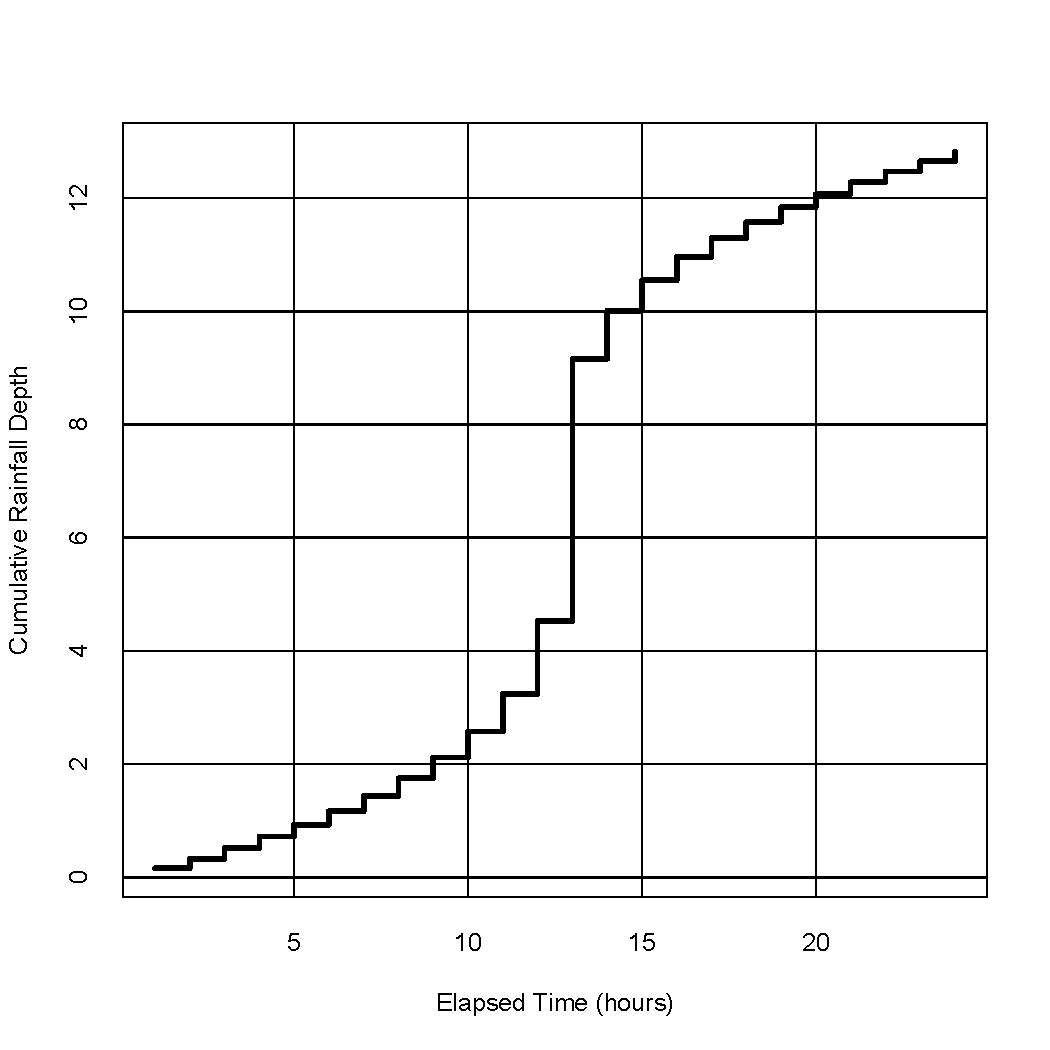
\includegraphics[width=5in]{accum_rain.pdf} 
   \caption{Cumulative rainfall for a 24-hour period on watershed determined for Figure \ref{fig:topoMap.jpg}}
   \label{fig:accum_rain.pdf}
\end{figure}

% Requires the booktabs if the memoir class is not being used
\begin{table}[htbp]
   \centering
   \caption{Cumulative Rainfall for Figure~\ref{fig:accum_rain.pdf}}
   \begin{tabular}{ccc} 
    Elapsed Time (hours)&Cum. Rainfall&Inc. Rainfall\\
    \hline
    \hline
      1&  0.16 & ~ \\
      2&  0.33 & ~ \\
      3 & 0.52 & ~ \\
      4&  0.72 & ~ \\
      5 & 0.93 & ~ \\
      6 & 1.17 & ~ \\
      7&  1.44 & ~ \\
      8&  1.75 & ~ \\
      9&  2.12 & ~ \\
    10 & 2.58 & ~ \\
    11&  3.24 & ~ \\
    12&  4.53 & ~ \\
    13 & 9.16 & ~ \\
    14& 10.01 & ~ \\
    15 &10.55 & ~ \\
    16 &10.96 & ~ \\
    17& 11.29 & ~ \\
    18& 11.58 & ~ \\
    19& 11.84 & ~ \\
    20& 12.07 & ~ \\
    21& 12.28 & ~ \\
    22& 12.47 & ~ \\
    23& 12.65 & ~ \\
   24& 12.82 & ~ \\
   \hline
   \end{tabular}

   \label{tab:rainfall}
\end{table}



\begin{figure}[h!] %  figure placement: here, top, bottom, or page
   \centering
   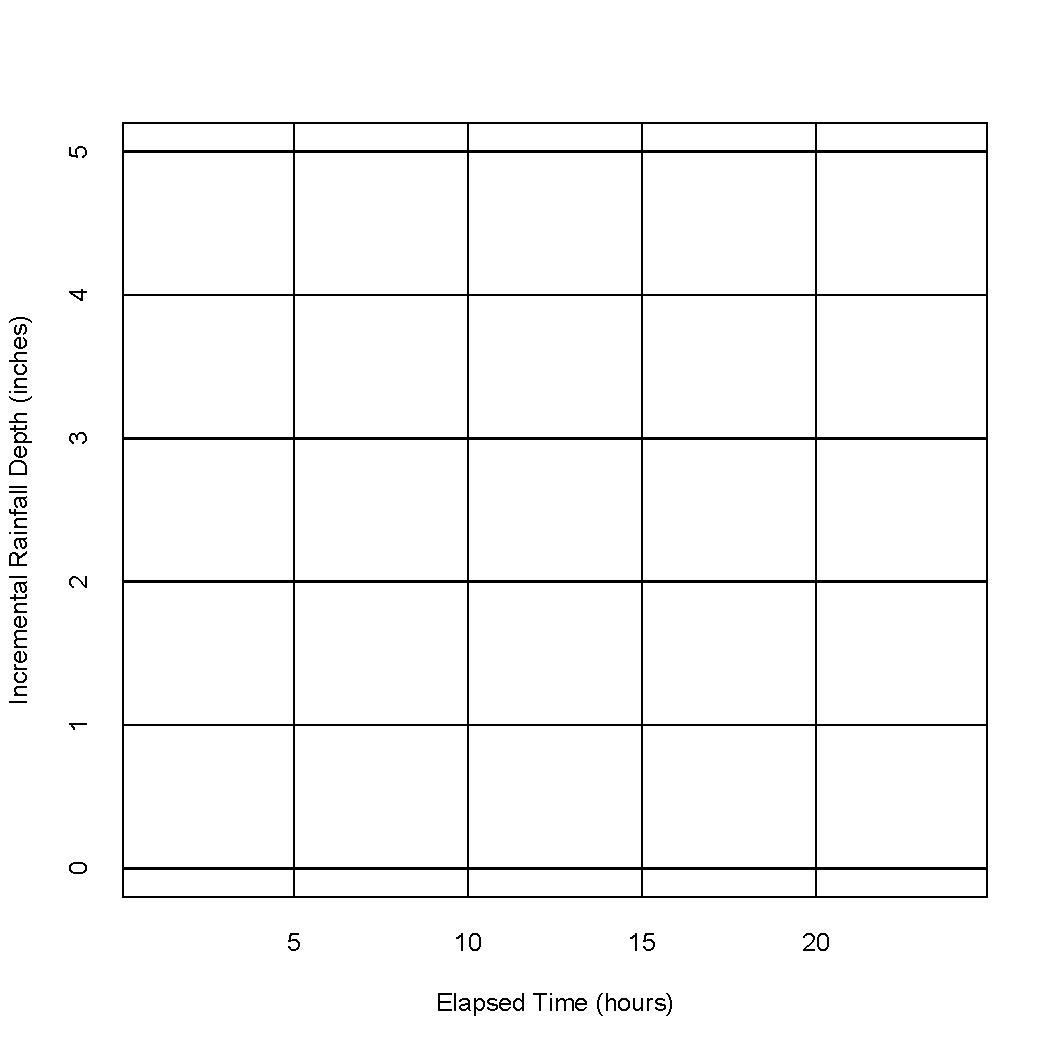
\includegraphics[width=5in]{incr_rain.pdf} 
   \caption{Incremental rainfall for a 24-hour period on watershed determined for Figure \ref{fig:topoMap.jpg}}
   \label{fig:incr_rain.pdf}
\end{figure}
%hours, depth
%1 ,0.16
%2 ,0.17
%3 ,0.19
%4 ,0.20
%5 ,0.21
%6 ,0.24
%7 ,0.27
%8 ,0.31
%9 ,0.37
%10 ,0.46
%11 ,0.66
%12 ,1.29
%13 ,4.63
%14 ,0.85
%15 ,0.54
%16 ,0.41
%17 ,0.33
%18 ,0.29
%19 ,0.26
%20 ,0.23
%21 ,0.21
%22 ,0.19
%23 ,0.18
%24 ,0.17
%============== PART 3 DESIGN STORM  ========================

\clearpage
\item Figure \ref{fig:hydrograph.jpg} is an observed runoff hydrograph at the watershed outlet (for the watershed in Figure ).  
  \begin{figure}[h!] %  figure placement: here, top, bottom, or page
   \centering
   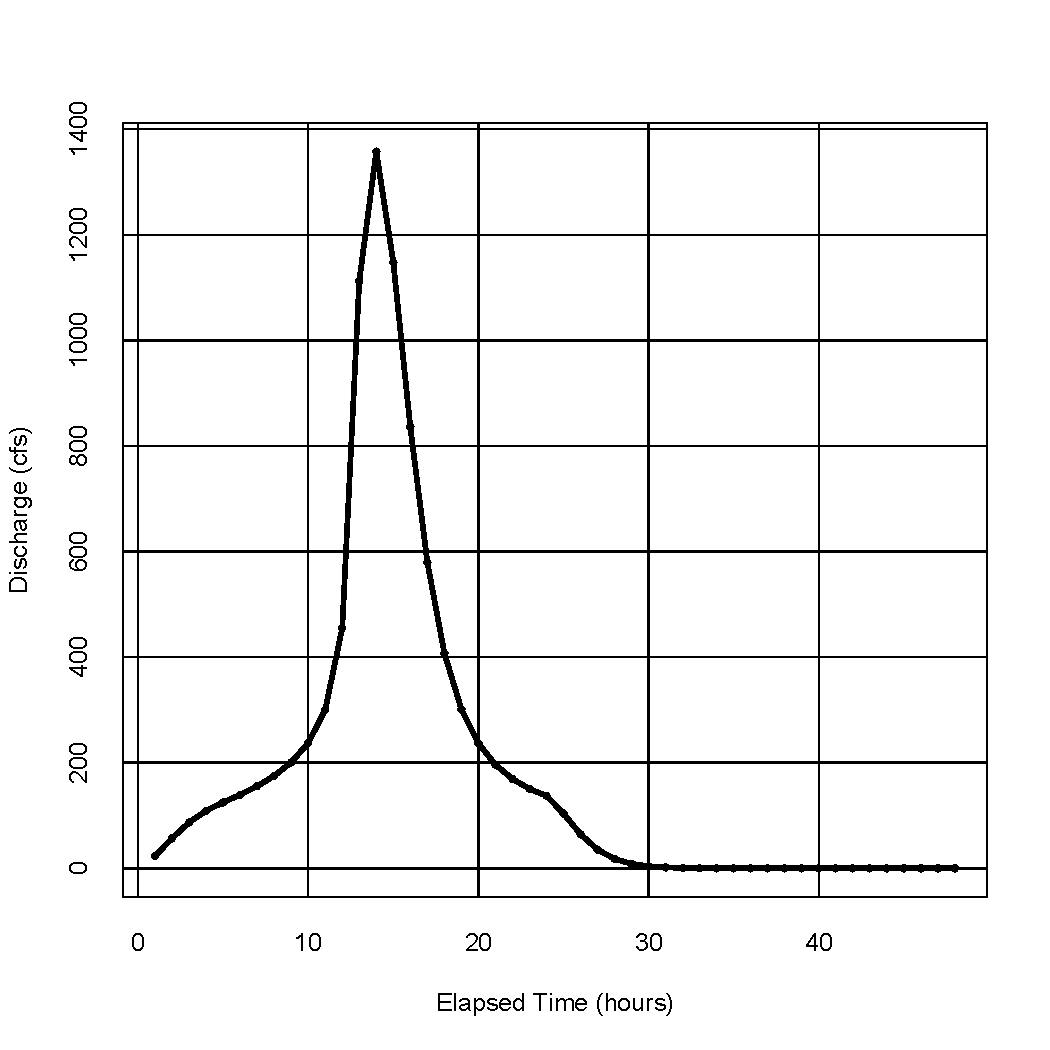
\includegraphics[width=5.5in]{hydrograph.pdf} 
   \caption{Observed runoff hydrograph for rainfall in Table~\ref{tab:rainfall} }
   \label{fig:hydrograph.jpg}
\end{figure}

Determine the following:

\begin{enumerate}[(a)]
\item What fraction of rainfall in total is converted into runoff?
\item What is the watershed response time from peak rainfall to peak runoff ?
%\item What is the estimated time based on the watershed physical characteristics ?
\end{enumerate}

%\textbf{If and only if time permits}
%
%\begin{enumerate}
%\item Develop a 24-hour Unit Hydrograph approximation from the rainfall and runoff data.  
%\item Estimate and sketch the response of the watershed to a 24-hour storm of the same pattern as presented here, except that the total depth is $\frac{1}{3}$ of the storm in Table~\ref{tab:rainfall}.
%\end{enumerate}

%  \begin{figure}[h!] %  figure placement: here, top, bottom, or page
%   \centering
%   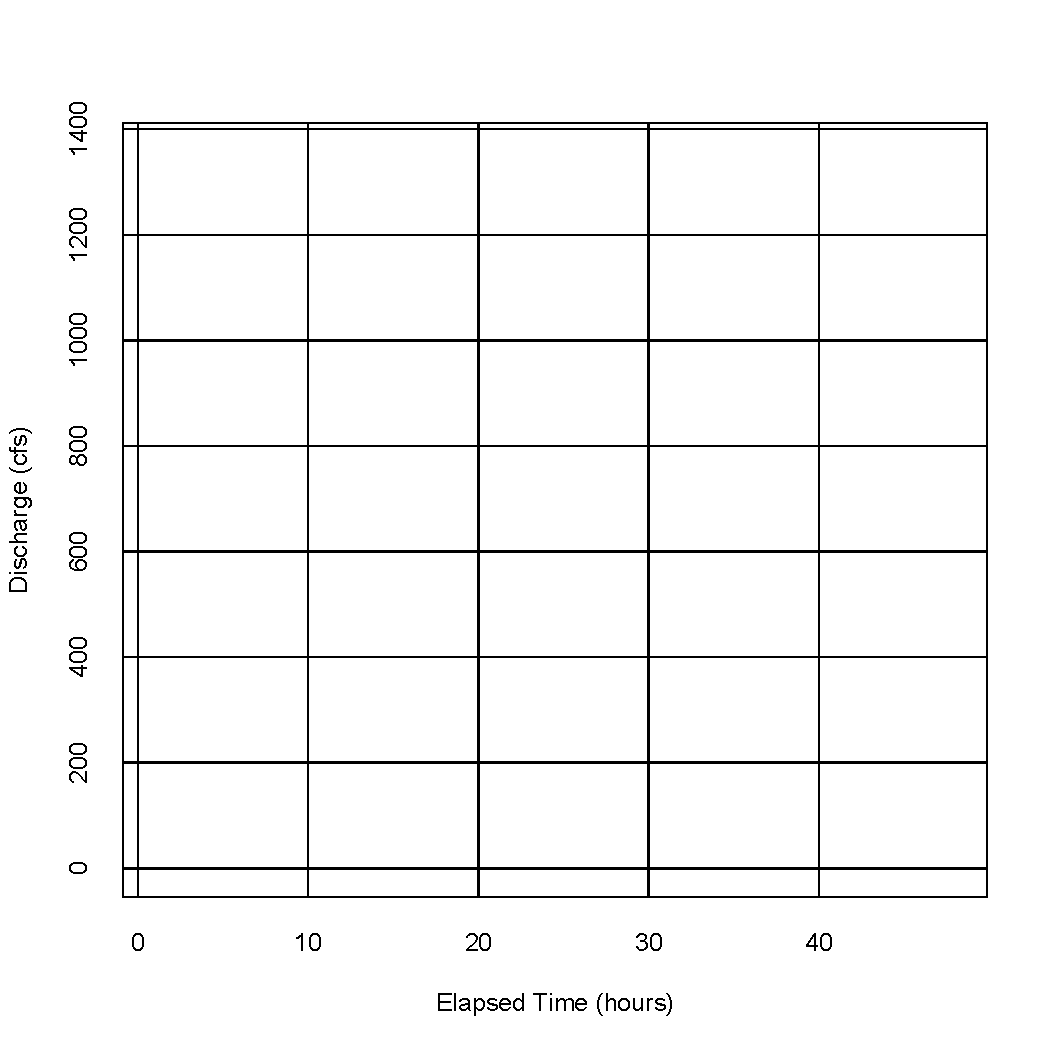
\includegraphics[width=5.5in]{blank_hydro.pdf} 
%   \caption{24-hour Unit Hydrograph and/or response hydrograph. (workspace)}
%   \label{fig:blank_hydro.jpg}
%\end{figure}

%============== PART 4 ROUTING (A TRICK) ===============
\newpage ~
Work Area
\clearpage

%Assume the dam in figure \ref{fig:topoMap.jpg} has been built and the pool level (elevation of water behind the dam) is at elevation $580~feet$.  Further assume an inter-basin drainage is built somewhere upstream so that the reservoir receives input from other than direct rainfall (on the reservoir).  
%  \begin{figure}[h!] %  figure placement: here, top, bottom, or page
%   \centering
%   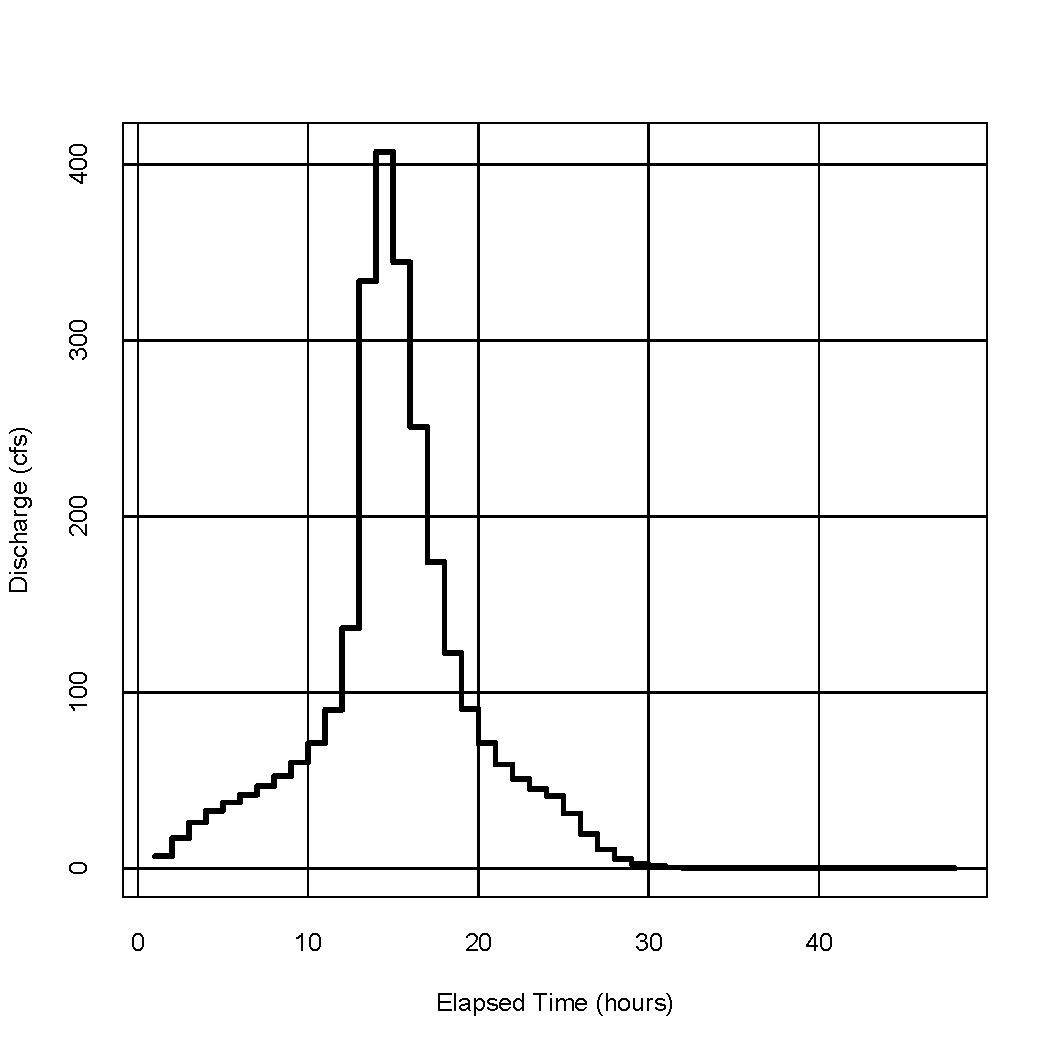
\includegraphics[width=5in]{input_hydro.pdf} 
%   \caption{Inter-basin input hydrograph.}
%   \label{fig:input_hydro.pdf}
%\end{figure}
%
%The reservoir is strictly uncontrolled and water exits only over the spillway.  The spillway elevation is $590~feet$.  Discharge through the spillway is given by
%\begin{equation}
%Q = 0.45 \sqrt{19.62} \times 10 H^{\frac{3}{2}}
%\end{equation}
%where $H$ is the height of water in $feet$ above the spillway elevation.  If $H$ is less than zero, then water is stored in the reservoir.
%
%Figure \ref{fig:input_hydro.pdf} is an input hydrograph from such an inter-basin connection.  Route this input hydrograph through the reservoir\footnote{Determine the outflow hydrograph at the reservoir outlet}.  
%
%\clearpage


\end{enumerate}

\end{document}




% ======== R CODE to generate figure ============
% z<-read.csv(file="rock_sizes.csv",header=T,as.is=F)
% attach(z)
% summary(z)
% ls<-LargeSize[1:30]
% plot(sort(SmallSize),seq(1,length(SmallSize))/(length(SmallSize)+1),pch=16,tck=1,xlim=c(0.2,2),log="x",xlab="Characteristic Length (inches)",ylab="Cum. Frequency");lines(sort(ls),seq(1,length(ls))/(length(ls)+1),pch=16,type="p",col="red")
% boxplot(SmallSize,ls,names=c("Small","Large"),xlab="Characteristic Length (inches)",horizontal=T)